\subsubsection{Current sensor} \label{current_sensor}

The current along with the voltage of the PV allows the system to perform power calculation, which is needed for the MPPT algorithm. The current will be measured in series with the inductor with a hall effect sensor. Placing it in series with the PV module would be the easiest approach for MPPT, but placing it in parallel with the inductor allows implementing a current controller for possible future use. A hall effect sensor is used to secure isolation between the power traces and the control circuit.

\begin{figure}[H]
	\begin{center}
		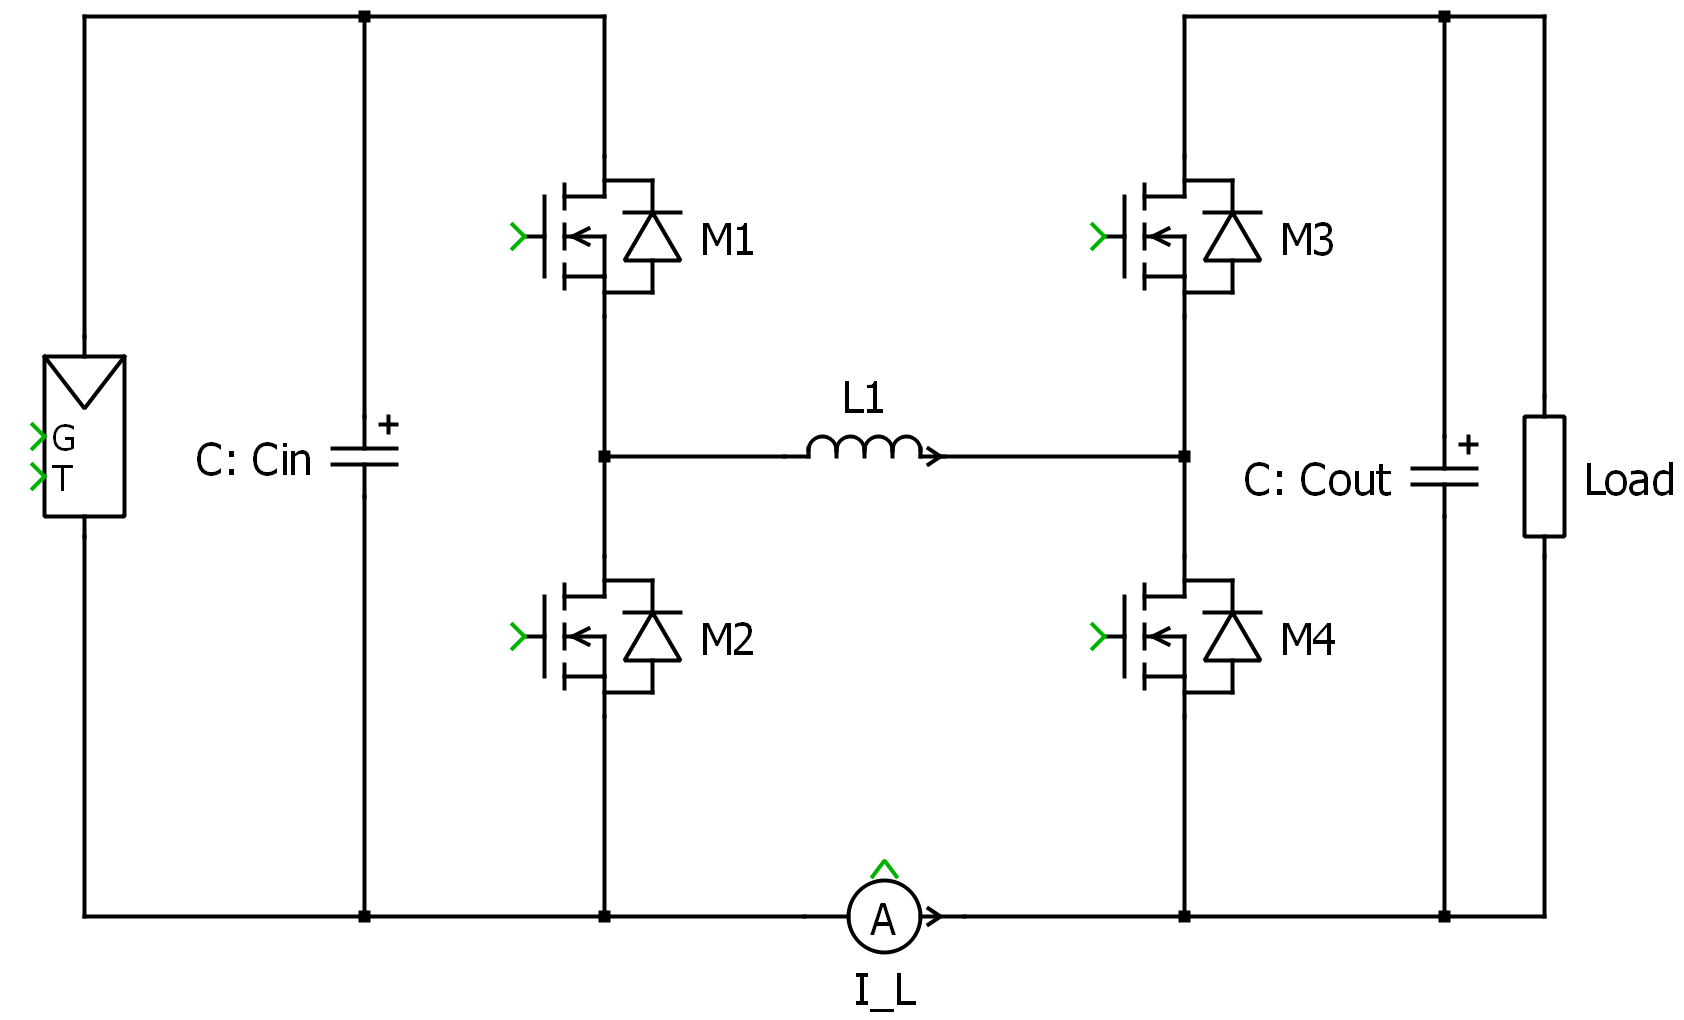
\includegraphics[width=0.5\textwidth]{../Pictures/current_sensor_placement.png}
		\caption{Current sensor placement.}
		\label{current_sensor_placement}
	\end{center}	
\end{figure}

The sensor is a ACS723-20AB \cite{current_sensor} which is a hall effect sensor. Its features can be found in table \ref{current_sensor_features} and its connection can be found in \ref{current_sensor_application}.

\begin{table}[H]
	\centering
	\begin{tabular}{|p{6cm}|>{\centering}p{8cm}|}
		\hline
		\rowcolor{lightgray}\multicolumn{2}{|l|}{ \textbf{Maximum ratings}} \\ \hline
		Supply voltage & 4.5-5.5 [V]  \tabularnewline \hline
		Gain & 100 [mV/A]  \tabularnewline \hline
		Input range & $\pm$20 [A]  \tabularnewline \hline
		\rowcolor{lightgray}\multicolumn{2}{|l|}{ \textbf{Other values of interest}} \\ \hline
		Bandwidth & 20 or 80 [kHz]  \tabularnewline \hline
		Package & SOIC8  \tabularnewline \hline
		
	\end{tabular}
	\caption{Current sensor figures of merit \cite{current_sensor}.}
	\label{current_sensor_features}
\end{table}

\begin{figure}[H]
	\begin{center}
		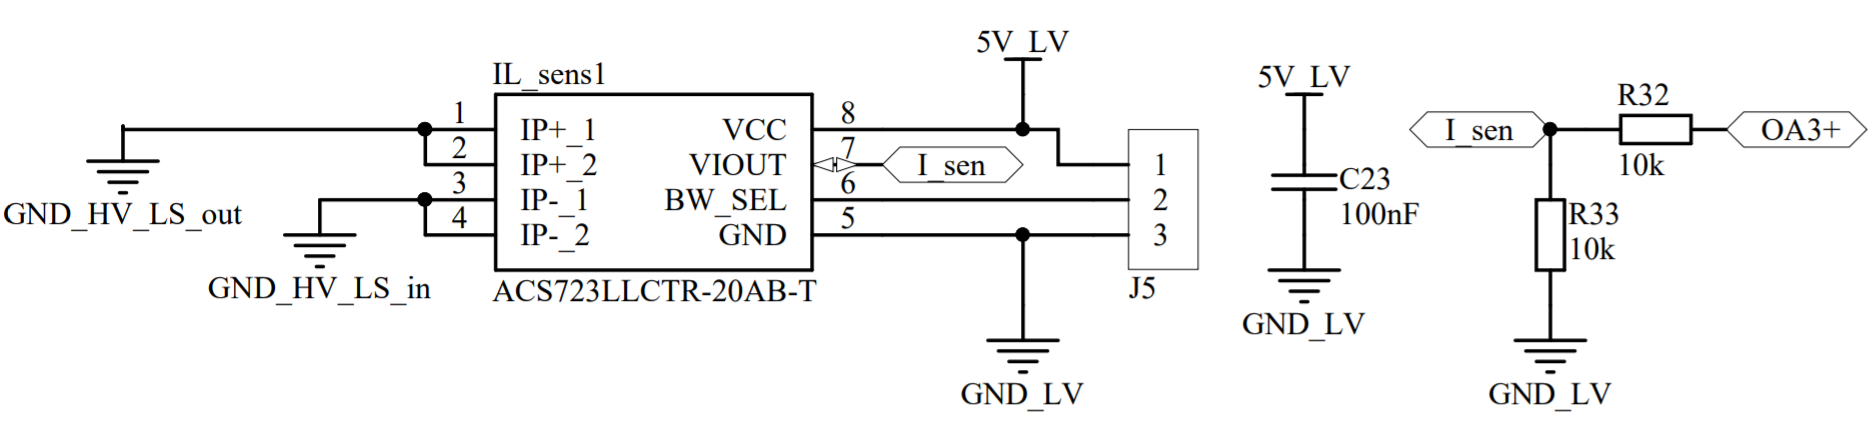
\includegraphics[width=\textwidth]{../Pictures/P1/Sensors/current_sensor}
		\caption{Current sensor connection.}
		\label{current_sensor_application}
	\end{center}	
\end{figure}

The output of the sensor is a voltage proportional to the current following the next equation:

\begin{equation} 
v_{current} = \frac{1}{10}V/A \cdot i + 2.5V
\end{equation}

In order to ease the task of the control, the signals are filtered by hardware. The current will be used by the MPPT, which frequency is $100 Hz$. The sensor output is filtered by a low-pass filter which cut-off frequency is $50 Hz$. Also the current might be used in the current controller, this signal will be filtered at $80 kHz$ in case a peak current controller is implemented. This cut-off frequency was selected as it is the sensor's bandwidth. The filters are first order low-pass filters implemented with a resistor in series with a capacitor.

In order to calculate the current from the PV module, the converter working mode will have to be taken into account. Assuming continuous conduction mode, the average PV current is:


\begin{equation} 
	Buck \; mode \rightarrow \overline{I_{in}} = \overline{i_{measured}} \cdot D
\end{equation}
\begin{equation} 
Boost \; mode \rightarrow \overline{I_{in}} = \overline{i_{measured}}
\end{equation}
\begin{equation} 
Buck-Boost \; mode \rightarrow \overline{I_{in}} = \overline{i_{measured}} \cdot D
\end{equation}